\newpage 
\thispagestyle{empty}
\chapter{Implementierung}\label{sec:Implementierung}
Wie im Kapitel \ref{sec:Interpretation_Dipol} erwähnt ist, wird die Antennenstruktur weder auf einer FR4 Kunstharzplatte noch auf eine Plastikfolie aufgedruckt. Da einerseits die Produktionskosten von Kleinserien im Verhältnis zum Nutzen eher klein sind, zum Andern benötigt jeder Fertigungsdurchgang von gedruckten Antennen  mindestens ein bis drei Tage. Daher werden die zu Testenden Antennen aus Kupferfolie geschnitten. So können Änderungen des Design sehr schnell umgesetzt werden und die Kosten sind gering.\\

Aus der Interpretation der Dipolantennen Simulationen \ref{sec:Interpretation_Dipol} ist hervorgegangen, dass das Abstrahlverhalten eine Dipolantenne mit einer Breite von 3 mm und einer Dicke von 26 $\mu m$ sowie einer Länge von 50.25 mm ausgemessen wird. Wie die Abbildung \ref{S11_Vergleich_Simulation_Dipolantenn_freiraum_Geraet} zeigt, unterscheidet sich das Abstrahlverhalten von Dipole mit einer Breite von 1 mm und 3 mm nur unfesentlich. Die Antennenstrucktur mit einer Breite von 3 mm ist wesentlich einfacher zu bearbeiten als die 1 mm Breiten Antennestruckturen. Das Kupferband mit einer Beite von weniger als 3 mm kann unter keinem Zug reissen. Zudem ist die grössere Klebefäche von Vorteil um die Antenne an das Kunststoffgehäuse zu fixieren.  \\
\newpage
Die Antenne wird mit dem Skalpell aus dem Kupferklebeband ausgeschnitten. Das ist in der Abbildung \ref{fig:DipolausKupferband} gezeigt. Dabei gilt es zu beachten, dass sich das Kupferband nicht in seine ursprünglicher Form zurück zieht. Das Zentrum der Antenne, dient als Fusspunkt der Antenne, dieser wird mit einem ca. 1 mm$^{2}$ grosssen Lötzinnpunkt versehen. An diesem speisst die Zuleitung, in Form eines Koaxialkabels, die Antenne.\\
\begin{figure}[!ht]
	\centering
	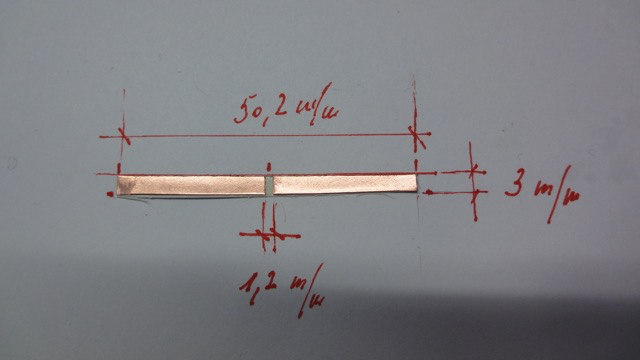
\includegraphics[width=13cm]{content/bilder/Implementierung/Dipol3mm50mm.jpg}%
	\caption{Dipol aus Kupferklebeband ausgeschnitten}
	\label{fig:DipolausKupferband}
\end{figure}
%\newpage

In der Abbildung \ref{fig:DipolausKupferbandGeraeteinnenseite} ist  die Dipolantenne mit einem Koaxialkabel als Speiseleitung gezeigt. Das Koaxialkabel diehnt als längs homogene Leiteung. Sie führt die elektromagnetische Welle von der Quelle zur Antenne. Die Leitung wird rechtwinklig von der Antenne weggeführt. Es muss stehts darauf geachtet werden, dass sich das der Biegeradius des Koaxialkabels einghalten wird. Der Aussenleiter des Koaxialkabels muss nicht zusätzlich gegenüber dem darunterliedenden Akkupaket isoliert werden. Denn diser ist bereits in eine Kunstofffolie gehüllt. Jedoch muss darauf geachtet werden, dass der Aussenleiter des Koaxialkabels, nicht mir der Elektronikplatione, die sich auf der Rückseite des Displays befindet, kurzschliesst. Daher erfüllt das Papierklebeband mehrere Aufgaben. Es dient als Isolation zwischen der Elektronikplatione und dem Koaxialkabel und zusähzlich als Zugsentlastung der Antenne. Des weitern hilft das Papierkelbeband zur Fixierung der Antenne.\\
\begin{figure}[!ht]
	\centering
	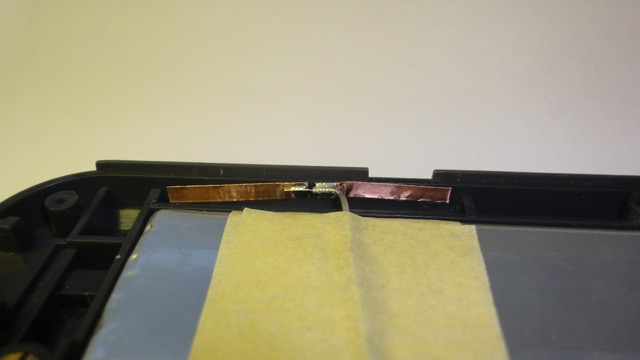
\includegraphics[width=13cm]{content/bilder/Implementierung/DipolIMGeraet.jpg}%
	\caption{Dipol aus Kupferklebeband an der Geräteinnenseite befestigt}
	\label{fig:DipolausKupferbandGeraeteinnenseite}
\end{figure}

\newpage
Die Abbildung \ref{fig:DipolimGeraet} zeigt wie die Antenne im Fluginstrumet positioniert ist. Auf diesr Abbildung ist sehr gut zu erkennen, dass die Antenne dirkt an die Aussenwand des Kuststoffgehöuse des Fluginstumetes geklebt ist. Das Koaxialkabel fühert rechtwinklig von der Antenne weg. Bis zum SMA Stecker, über diesen wird die Antenne mit der interen Quelle des Starlab verbunden.\\
\begin{figure}[!ht]
	\centering
	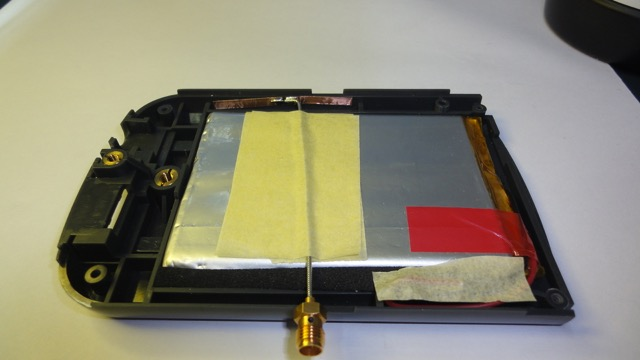
\includegraphics[width=13cm]{content/bilder/Implementierung/DipolKabelGeraet.jpg}%
	\caption{Dipol im Geraet und Koaxialkabel}
	\label{fig:DipolimGeraet}
\end{figure}

\newpage
Aus den Simulationen ind er Abbildung \ref{S11_Vergleich_Simulation_Dipolantenn_freiraum_Geraet} ist der |$S_{11}$| Verlauf im Freiraum und im Gerät bekannt. Die nachfolgende Abbildung zeigt als rote Kurve den $S_{11}$ Wert der Dipolantenne im Freiraum. Als rote Kurve ist der Verlauf des $S_{11}$ gezeigt, wenn die Dipolantenne im Gerät positioniert ist. Es ist die breits erwähnte Verschiebung der Resonanzfrequenz ersichtlicht. Zudem ist die Resonanz der Dämpfung des $S_{11}$ Verlaufs im Gerät weniger stark ausgeprägt wie im Freiraum. Die Messung der im Gerät platzierten Dipolantenne ist als grüne Kurve in der Abbildung \ref{S11_Messung_Simulation_Dipolantenn_Freiraum} dargestellt. Die Resonaz der bluen Kurve(Simulation des Dipols im Gerät) und die Resonaz der grünen Kurve(Messung des Dipols im Gerät) stimmen gut überein. Was erstaunt, ist dass die $S_{11}$ Dämpfung der zuführenden Welle -15dB aufweisst. Ein erklährungsversuch weisst auf das Simulationsmodell. Es zeigt qualitativ wie wie sich die Resonazfrequenz von einem Dipol im Freiraum gegenüber einem Dipol im Gerät verhält. Es macht aber erhebliche Fehler beim Impedanzverhalten. So weisst der gemessene Dipol bei einer Frequenz von 2.45 GHz eine Antennenimpedanz von $Z_{ant}$ = (30+j4)$\Omega$. Während aus der Simulation die Antennenimpedanz von $Z_{ant}$ = (16+j14.7)$\Omega$ aus Tabelle \ref{tab:Vergeich_Lambda/2_Freiraum_Geraet} zu entnehmen ist. Demnach ist die Anpassung von an eine 50$\Omega$ Quelle in realität bersser als aus der Simulation erwartet.


%\begin{figure}[!ht]
%	\centering
%	\begingroup
%	\inputencoding{latin1}
%	\input{content/bilder/Messung/Messung_Sim_S11_Freiraum.tikz}
%	\endgroup
%	\caption{Vergleich des gemessen und simulierten $S_{11}$ Werts im Freiraum}	\label{S11_Messung_Simulation_Dipolantenn_Freiraum}
%\end{figure}

\begin{figure}[!ht]
	\centering
	\begingroup
	\inputencoding{latin1}
	% This file was created by matlab2tikz.
%
%The latest updates can be retrieved from
%  http://www.mathworks.com/matlabcentral/fileexchange/22022-matlab2tikz-matlab2tikz
%where you can also make suggestions and rate matlab2tikz.
%
\begin{tikzpicture}

\begin{axis}[%
width=6in,
height=4in,
at={(1.123in,0.757in)},
scale only axis,
separate axis lines,
every outer x axis line/.append style={black},
every x tick label/.append style={font=\color{black}},
xmin=2000000000,
xmax=3000000000,
xlabel={Frequenz in [Hz]},
xmajorgrids,
every outer y axis line/.append style={black},
every y tick label/.append style={font=\color{black}},
ymin=-16,
ymax=0,
ylabel={Amplitude in [dB]},
ymajorgrids,
axis background/.style={fill=white},
title={$\text{Simulation des  S}_{\text{11}}\text{ im Freiraum und dim Ger\"at eines Dipol 3 mm breit}$},
legend style={at={(0.99,0.01)},anchor=south east,legend cell align=left,align=left,draw=black}
]
\addplot [color=red,solid,line width=2.0pt]
  table[row sep=crcr]{%
2000000000	-2.27999\\
2001670000	-2.29471\\
2003330000	-2.30952\\
2005000000	-2.32443\\
2006670000	-2.33943\\
2008330000	-2.35453\\
2010000000	-2.36973\\
2011670000	-2.38502\\
2013330000	-2.40041\\
2015000000	-2.4159\\
2016670000	-2.43149\\
2018330000	-2.44717\\
2020000000	-2.46296\\
2021670000	-2.47885\\
2023330000	-2.49484\\
2025000000	-2.51093\\
2026670000	-2.52712\\
2028330000	-2.54342\\
2030000000	-2.55982\\
2031670000	-2.57633\\
2033330000	-2.59294\\
2035000000	-2.60965\\
2036670000	-2.62647\\
2038330000	-2.6434\\
2040000000	-2.66044\\
2041670000	-2.67758\\
2043330000	-2.69483\\
2045000000	-2.7122\\
2046670000	-2.72967\\
2048330000	-2.74725\\
2050000000	-2.76495\\
2051670000	-2.78275\\
2053330000	-2.80067\\
2055000000	-2.8187\\
2056670000	-2.83685\\
2058330000	-2.85511\\
2060000000	-2.87348\\
2061670000	-2.89197\\
2063330000	-2.91058\\
2065000000	-2.92931\\
2066670000	-2.94815\\
2068330000	-2.96711\\
2070000000	-2.98619\\
2071670000	-3.00539\\
2073330000	-3.02471\\
2075000000	-3.04415\\
2076670000	-3.06371\\
2078330000	-3.0834\\
2080000000	-3.10321\\
2081670000	-3.12314\\
2083330000	-3.1432\\
2085000000	-3.16338\\
2086670000	-3.18369\\
2088330000	-3.20413\\
2090000000	-3.22469\\
2091670000	-3.24538\\
2093330000	-3.2662\\
2095000000	-3.28715\\
2096670000	-3.30823\\
2098330000	-3.32944\\
2100000000	-3.35078\\
2101670000	-3.37225\\
2103330000	-3.39386\\
2105000000	-3.4156\\
2106670000	-3.43748\\
2108330000	-3.45949\\
2110000000	-3.48163\\
2111670000	-3.50392\\
2113330000	-3.52634\\
2115000000	-3.54889\\
2116670000	-3.57159\\
2118330000	-3.59443\\
2120000000	-3.61741\\
2121670000	-3.64052\\
2123330000	-3.66378\\
2125000000	-3.68718\\
2126670000	-3.71073\\
2128330000	-3.73442\\
2130000000	-3.75825\\
2131670000	-3.78223\\
2133330000	-3.80636\\
2135000000	-3.83063\\
2136670000	-3.85505\\
2138330000	-3.87962\\
2140000000	-3.90433\\
2141670000	-3.9292\\
2143330000	-3.95422\\
2145000000	-3.97939\\
2146670000	-4.00471\\
2148330000	-4.03018\\
2150000000	-4.05581\\
2151670000	-4.08159\\
2153330000	-4.10753\\
2155000000	-4.13362\\
2156670000	-4.15987\\
2158330000	-4.18628\\
2160000000	-4.21284\\
2161670000	-4.23956\\
2163330000	-4.26645\\
2165000000	-4.29349\\
2166670000	-4.3207\\
2168330000	-4.34806\\
2170000000	-4.37559\\
2171670000	-4.40329\\
2173330000	-4.43114\\
2175000000	-4.45916\\
2176670000	-4.48735\\
2178330000	-4.51571\\
2180000000	-4.54423\\
2181670000	-4.57291\\
2183330000	-4.60177\\
2185000000	-4.6308\\
2186670000	-4.66\\
2188330000	-4.68936\\
2190000000	-4.7189\\
2191670000	-4.74862\\
2193330000	-4.7785\\
2195000000	-4.80856\\
2196670000	-4.83879\\
2198330000	-4.8692\\
2200000000	-4.89979\\
2201670000	-4.93055\\
2203330000	-4.96149\\
2205000000	-4.9926\\
2206670000	-5.0239\\
2208330000	-5.05537\\
2210000000	-5.08703\\
2211670000	-5.11887\\
2213330000	-5.15088\\
2215000000	-5.18308\\
2216670000	-5.21547\\
2218330000	-5.24803\\
2220000000	-5.28079\\
2221670000	-5.31372\\
2223330000	-5.34685\\
2225000000	-5.38015\\
2226670000	-5.41365\\
2228330000	-5.44733\\
2230000000	-5.48121\\
2231670000	-5.51527\\
2233330000	-5.54952\\
2235000000	-5.58396\\
2236670000	-5.61859\\
2238330000	-5.65341\\
2240000000	-5.68843\\
2241670000	-5.72364\\
2243330000	-5.75904\\
2245000000	-5.79463\\
2246670000	-5.83042\\
2248330000	-5.8664\\
2250000000	-5.90258\\
2251670000	-5.93896\\
2253330000	-5.97553\\
2255000000	-6.0123\\
2256670000	-6.04926\\
2258330000	-6.08643\\
2260000000	-6.12379\\
2261670000	-6.16135\\
2263330000	-6.19911\\
2265000000	-6.23707\\
2266670000	-6.27523\\
2268330000	-6.31359\\
2270000000	-6.35215\\
2271670000	-6.39091\\
2273330000	-6.42988\\
2275000000	-6.46904\\
2276670000	-6.50841\\
2278330000	-6.54798\\
2280000000	-6.58775\\
2281670000	-6.62772\\
2283330000	-6.6679\\
2285000000	-6.70828\\
2286670000	-6.74886\\
2288330000	-6.78965\\
2290000000	-6.83064\\
2291670000	-6.87183\\
2293330000	-6.91323\\
2295000000	-6.95483\\
2296670000	-6.99663\\
2298330000	-7.03864\\
2300000000	-7.08085\\
2301670000	-7.12326\\
2303330000	-7.16588\\
2305000000	-7.2087\\
2306670000	-7.25172\\
2308330000	-7.29494\\
2310000000	-7.33837\\
2311670000	-7.382\\
2313330000	-7.42582\\
2315000000	-7.46985\\
2316670000	-7.51408\\
2318330000	-7.55851\\
2320000000	-7.60314\\
2321670000	-7.64796\\
2323330000	-7.69299\\
2325000000	-7.73821\\
2326670000	-7.78362\\
2328330000	-7.82923\\
2330000000	-7.87504\\
2331670000	-7.92104\\
2333330000	-7.96723\\
2335000000	-8.01361\\
2336670000	-8.06018\\
2338330000	-8.10694\\
2340000000	-8.15389\\
2341670000	-8.20102\\
2343330000	-8.24834\\
2345000000	-8.29584\\
2346670000	-8.34352\\
2348330000	-8.39138\\
2350000000	-8.43941\\
2351670000	-8.48763\\
2353330000	-8.53601\\
2355000000	-8.58457\\
2356670000	-8.63329\\
2358330000	-8.68219\\
2360000000	-8.73124\\
2361670000	-8.78046\\
2363330000	-8.82984\\
2365000000	-8.87937\\
2366670000	-8.92906\\
2368330000	-8.97889\\
2370000000	-9.02888\\
2371670000	-9.079\\
2373330000	-9.12927\\
2375000000	-9.17967\\
2376670000	-9.23021\\
2378330000	-9.28087\\
2380000000	-9.33167\\
2381670000	-9.38258\\
2383330000	-9.43361\\
2385000000	-9.48475\\
2386670000	-9.53599\\
2388330000	-9.58734\\
2390000000	-9.63879\\
2391670000	-9.69033\\
2393330000	-9.74196\\
2395000000	-9.79367\\
2396670000	-9.84545\\
2398330000	-9.89731\\
2400000000	-9.94922\\
2401670000	-10.0012\\
2403330000	-10.0532\\
2405000000	-10.1053\\
2406670000	-10.1574\\
2408330000	-10.2095\\
2410000000	-10.2617\\
2411670000	-10.3139\\
2413330000	-10.366\\
2415000000	-10.4182\\
2416670000	-10.4704\\
2418330000	-10.5225\\
2420000000	-10.5747\\
2421670000	-10.6267\\
2423330000	-10.6788\\
2425000000	-10.7308\\
2426670000	-10.7827\\
2428330000	-10.8345\\
2430000000	-10.8863\\
2431670000	-10.9379\\
2433330000	-10.9895\\
2435000000	-11.0409\\
2436670000	-11.0922\\
2438330000	-11.1433\\
2440000000	-11.1943\\
2441670000	-11.2451\\
2443330000	-11.2958\\
2445000000	-11.3462\\
2446670000	-11.3965\\
2448330000	-11.4465\\
2450000000	-11.4963\\
2451670000	-11.5458\\
2453330000	-11.5951\\
2455000000	-11.644\\
2456670000	-11.6927\\
2458330000	-11.7411\\
2460000000	-11.7892\\
2461670000	-11.8369\\
2463330000	-11.8843\\
2465000000	-11.9312\\
2466670000	-11.9778\\
2468330000	-12.024\\
2470000000	-12.0698\\
2471670000	-12.1151\\
2473330000	-12.16\\
2475000000	-12.2044\\
2476670000	-12.2483\\
2478330000	-12.2917\\
2480000000	-12.3346\\
2481670000	-12.3769\\
2483330000	-12.4186\\
2485000000	-12.4598\\
2486670000	-12.5004\\
2488330000	-12.5404\\
2490000000	-12.5797\\
2491670000	-12.6184\\
2493330000	-12.6564\\
2495000000	-12.6937\\
2496670000	-12.7303\\
2498330000	-12.7662\\
2500000000	-12.8013\\
2501670000	-12.8357\\
2503330000	-12.8693\\
2505000000	-12.9021\\
2506670000	-12.9341\\
2508330000	-12.9653\\
2510000000	-12.9956\\
2511670000	-13.0251\\
2513330000	-13.0537\\
2515000000	-13.0815\\
2516670000	-13.1083\\
2518330000	-13.1342\\
2520000000	-13.1592\\
2521670000	-13.1833\\
2523330000	-13.2064\\
2525000000	-13.2285\\
2526670000	-13.2497\\
2528330000	-13.2699\\
2530000000	-13.2891\\
2531670000	-13.3073\\
2533330000	-13.3245\\
2535000000	-13.3407\\
2536670000	-13.3558\\
2538330000	-13.3699\\
2540000000	-13.383\\
2541670000	-13.3951\\
2543330000	-13.4061\\
2545000000	-13.4161\\
2546670000	-13.4251\\
2548330000	-13.433\\
2550000000	-13.4398\\
2551670000	-13.4456\\
2553330000	-13.4504\\
2555000000	-13.4541\\
2556670000	-13.4568\\
2558330000	-13.4585\\
2560000000	-13.4591\\
2561670000	-13.4587\\
2563330000	-13.4573\\
2565000000	-13.4549\\
2566670000	-13.4515\\
2568330000	-13.4471\\
2570000000	-13.4417\\
2571670000	-13.4354\\
2573330000	-13.428\\
2575000000	-13.4198\\
2576670000	-13.4106\\
2578330000	-13.4004\\
2580000000	-13.3894\\
2581670000	-13.3774\\
2583330000	-13.3646\\
2585000000	-13.3509\\
2586670000	-13.3363\\
2588330000	-13.3209\\
2590000000	-13.3046\\
2591670000	-13.2876\\
2593330000	-13.2697\\
2595000000	-13.2511\\
2596670000	-13.2317\\
2598330000	-13.2115\\
2600000000	-13.1906\\
2601670000	-13.169\\
2603330000	-13.1468\\
2605000000	-13.1238\\
2606670000	-13.1002\\
2608330000	-13.0759\\
2610000000	-13.051\\
2611670000	-13.0255\\
2613330000	-12.9994\\
2615000000	-12.9727\\
2616670000	-12.9455\\
2618330000	-12.9177\\
2620000000	-12.8894\\
2621670000	-12.8606\\
2623330000	-12.8313\\
2625000000	-12.8015\\
2626670000	-12.7713\\
2628330000	-12.7407\\
2630000000	-12.7096\\
2631670000	-12.6781\\
2633330000	-12.6462\\
2635000000	-12.614\\
2636670000	-12.5814\\
2638330000	-12.5484\\
2640000000	-12.5151\\
2641670000	-12.4815\\
2643330000	-12.4476\\
2645000000	-12.4135\\
2646670000	-12.379\\
2648330000	-12.3443\\
2650000000	-12.3093\\
2651670000	-12.2741\\
2653330000	-12.2387\\
2655000000	-12.2031\\
2656670000	-12.1673\\
2658330000	-12.1313\\
2660000000	-12.0951\\
2661670000	-12.0588\\
2663330000	-12.0223\\
2665000000	-11.9857\\
2666670000	-11.9489\\
2668330000	-11.9121\\
2670000000	-11.8751\\
2671670000	-11.838\\
2673330000	-11.8009\\
2675000000	-11.7636\\
2676670000	-11.7263\\
2678330000	-11.6889\\
2680000000	-11.6515\\
2681670000	-11.6141\\
2683330000	-11.5765\\
2685000000	-11.539\\
2686670000	-11.5014\\
2688330000	-11.4639\\
2690000000	-11.4263\\
2691670000	-11.3887\\
2693330000	-11.3511\\
2695000000	-11.3135\\
2696670000	-11.276\\
2698330000	-11.2385\\
2700000000	-11.201\\
2701670000	-11.1635\\
2703330000	-11.1261\\
2705000000	-11.0887\\
2706670000	-11.0513\\
2708330000	-11.0141\\
2710000000	-10.9768\\
2711670000	-10.9397\\
2713330000	-10.9026\\
2715000000	-10.8656\\
2716670000	-10.8286\\
2718330000	-10.7918\\
2720000000	-10.755\\
2721670000	-10.7183\\
2723330000	-10.6817\\
2725000000	-10.6452\\
2726670000	-10.6087\\
2728330000	-10.5724\\
2730000000	-10.5362\\
2731670000	-10.5001\\
2733330000	-10.4641\\
2735000000	-10.4282\\
2736670000	-10.3924\\
2738330000	-10.3567\\
2740000000	-10.3211\\
2741670000	-10.2857\\
2743330000	-10.2504\\
2745000000	-10.2152\\
2746670000	-10.1801\\
2748330000	-10.1451\\
2750000000	-10.1103\\
2751670000	-10.0756\\
2753330000	-10.0411\\
2755000000	-10.0066\\
2756670000	-9.9723\\
2758330000	-9.93813\\
2760000000	-9.90409\\
2761670000	-9.87018\\
2763330000	-9.83641\\
2765000000	-9.80278\\
2766670000	-9.76928\\
2768330000	-9.73592\\
2770000000	-9.7027\\
2771670000	-9.66962\\
2773330000	-9.63669\\
2775000000	-9.60389\\
2776670000	-9.57123\\
2778330000	-9.53872\\
2780000000	-9.50635\\
2781670000	-9.47412\\
2783330000	-9.44203\\
2785000000	-9.41009\\
2786670000	-9.37829\\
2788330000	-9.34663\\
2790000000	-9.31512\\
2791670000	-9.28375\\
2793330000	-9.25253\\
2795000000	-9.22145\\
2796670000	-9.19051\\
2798330000	-9.15972\\
2800000000	-9.12907\\
2801670000	-9.09857\\
2803330000	-9.06821\\
2805000000	-9.038\\
2806670000	-9.00792\\
2808330000	-8.978\\
2810000000	-8.94821\\
2811670000	-8.91857\\
2813330000	-8.88907\\
2815000000	-8.85971\\
2816670000	-8.8305\\
2818330000	-8.80143\\
2820000000	-8.7725\\
2821670000	-8.74371\\
2823330000	-8.71506\\
2825000000	-8.68655\\
2826670000	-8.65819\\
2828330000	-8.62996\\
2830000000	-8.60187\\
2831670000	-8.57392\\
2833330000	-8.54611\\
2835000000	-8.51844\\
2836670000	-8.49091\\
2838330000	-8.46351\\
2840000000	-8.43625\\
2841670000	-8.40912\\
2843330000	-8.38214\\
2845000000	-8.35528\\
2846670000	-8.32856\\
2848330000	-8.30198\\
2850000000	-8.27553\\
2851670000	-8.24921\\
2853330000	-8.22303\\
2855000000	-8.19697\\
2856670000	-8.17105\\
2858330000	-8.14526\\
2860000000	-8.1196\\
2861670000	-8.09407\\
2863330000	-8.06867\\
2865000000	-8.04339\\
2866670000	-8.01825\\
2868330000	-7.99323\\
2870000000	-7.96834\\
2871670000	-7.94358\\
2873330000	-7.91894\\
2875000000	-7.89442\\
2876670000	-7.87003\\
2878330000	-7.84577\\
2880000000	-7.82163\\
2881670000	-7.79761\\
2883330000	-7.77371\\
2885000000	-7.74993\\
2886670000	-7.72627\\
2888330000	-7.70274\\
2890000000	-7.67932\\
2891670000	-7.65602\\
2893330000	-7.63284\\
2895000000	-7.60978\\
2896670000	-7.58684\\
2898330000	-7.56401\\
2900000000	-7.54129\\
2901670000	-7.51869\\
2903330000	-7.49621\\
2905000000	-7.47384\\
2906670000	-7.45158\\
2908330000	-7.42944\\
2910000000	-7.40741\\
2911670000	-7.38549\\
2913330000	-7.36368\\
2915000000	-7.34198\\
2916670000	-7.32039\\
2918330000	-7.2989\\
2920000000	-7.27753\\
2921670000	-7.25626\\
2923330000	-7.23511\\
2925000000	-7.21405\\
2926670000	-7.19311\\
2928330000	-7.17227\\
2930000000	-7.15153\\
2931670000	-7.1309\\
2933330000	-7.11037\\
2935000000	-7.08994\\
2936670000	-7.06962\\
2938330000	-7.0494\\
2940000000	-7.02928\\
2941670000	-7.00926\\
2943330000	-6.98934\\
2945000000	-6.96952\\
2946670000	-6.94979\\
2948330000	-6.93017\\
2950000000	-6.91064\\
2951670000	-6.89121\\
2953330000	-6.87188\\
2955000000	-6.85264\\
2956670000	-6.8335\\
2958330000	-6.81445\\
2960000000	-6.7955\\
2961670000	-6.77664\\
2963330000	-6.75787\\
2965000000	-6.7392\\
2966670000	-6.72062\\
2968330000	-6.70213\\
2970000000	-6.68373\\
2971670000	-6.66542\\
2973330000	-6.6472\\
2975000000	-6.62907\\
2976670000	-6.61103\\
2978330000	-6.59307\\
2980000000	-6.57521\\
2981670000	-6.55743\\
2983330000	-6.53974\\
2985000000	-6.52213\\
2986670000	-6.50461\\
2988330000	-6.48718\\
2990000000	-6.46983\\
2991670000	-6.45256\\
2993330000	-6.43538\\
2995000000	-6.41828\\
2996670000	-6.40126\\
2998330000	-6.38433\\
3000000000	-6.36748\\
};
\addlegendentry{$\text{S}_{\text{11}}\text{ Frei Raum}$};

\addplot [color=blue,solid,line width=2.0pt]
  table[row sep=crcr]{%
2000000000	-0.594386\\
2001670000	-0.600369\\
2003330000	-0.606414\\
2005000000	-0.612525\\
2006670000	-0.618701\\
2008330000	-0.624943\\
2010000000	-0.631251\\
2011670000	-0.637628\\
2013330000	-0.644072\\
2015000000	-0.650586\\
2016670000	-0.657169\\
2018330000	-0.663823\\
2020000000	-0.670549\\
2021670000	-0.677347\\
2023330000	-0.684217\\
2025000000	-0.691162\\
2026670000	-0.698181\\
2028330000	-0.705276\\
2030000000	-0.712446\\
2031670000	-0.719694\\
2033330000	-0.72702\\
2035000000	-0.734425\\
2036670000	-0.74191\\
2038330000	-0.749475\\
2040000000	-0.757122\\
2041670000	-0.764851\\
2043330000	-0.772663\\
2045000000	-0.78056\\
2046670000	-0.788541\\
2048330000	-0.796609\\
2050000000	-0.804764\\
2051670000	-0.813006\\
2053330000	-0.821338\\
2055000000	-0.829759\\
2056670000	-0.838271\\
2058330000	-0.846874\\
2060000000	-0.855571\\
2061670000	-0.864361\\
2063330000	-0.873246\\
2065000000	-0.882227\\
2066670000	-0.891304\\
2068330000	-0.90048\\
2070000000	-0.909754\\
2071670000	-0.919128\\
2073330000	-0.928603\\
2075000000	-0.93818\\
2076670000	-0.94786\\
2078330000	-0.957644\\
2080000000	-0.967533\\
2081670000	-0.977528\\
2083330000	-0.987631\\
2085000000	-0.997843\\
2086670000	-1.00816\\
2088330000	-1.01859\\
2090000000	-1.02914\\
2091670000	-1.03979\\
2093330000	-1.05057\\
2095000000	-1.06145\\
2096670000	-1.07245\\
2098330000	-1.08357\\
2100000000	-1.09481\\
2101670000	-1.10617\\
2103330000	-1.11765\\
2105000000	-1.12925\\
2106670000	-1.14097\\
2108330000	-1.15282\\
2110000000	-1.1648\\
2111670000	-1.1769\\
2113330000	-1.18913\\
2115000000	-1.20149\\
2116670000	-1.21398\\
2118330000	-1.2266\\
2120000000	-1.23935\\
2121670000	-1.25224\\
2123330000	-1.26526\\
2125000000	-1.27842\\
2126670000	-1.29172\\
2128330000	-1.30515\\
2130000000	-1.31873\\
2131670000	-1.33245\\
2133330000	-1.34631\\
2135000000	-1.36031\\
2136670000	-1.37446\\
2138330000	-1.38876\\
2140000000	-1.4032\\
2141670000	-1.41779\\
2143330000	-1.43253\\
2145000000	-1.44742\\
2146670000	-1.46246\\
2148330000	-1.47766\\
2150000000	-1.49301\\
2151670000	-1.50851\\
2153330000	-1.52418\\
2155000000	-1.54\\
2156670000	-1.55598\\
2158330000	-1.57211\\
2160000000	-1.58841\\
2161670000	-1.60487\\
2163330000	-1.6215\\
2165000000	-1.63829\\
2166670000	-1.65524\\
2168330000	-1.67236\\
2170000000	-1.68965\\
2171670000	-1.7071\\
2173330000	-1.72473\\
2175000000	-1.74252\\
2176670000	-1.76049\\
2178330000	-1.77862\\
2180000000	-1.79693\\
2181670000	-1.81542\\
2183330000	-1.83407\\
2185000000	-1.8529\\
2186670000	-1.87191\\
2188330000	-1.89109\\
2190000000	-1.91046\\
2191670000	-1.92999\\
2193330000	-1.94971\\
2195000000	-1.9696\\
2196670000	-1.98968\\
2198330000	-2.00993\\
2200000000	-2.03036\\
2201670000	-2.05098\\
2203330000	-2.07177\\
2205000000	-2.09275\\
2206670000	-2.11391\\
2208330000	-2.13524\\
2210000000	-2.15676\\
2211670000	-2.17846\\
2213330000	-2.20035\\
2215000000	-2.22241\\
2216670000	-2.24465\\
2218330000	-2.26708\\
2220000000	-2.28968\\
2221670000	-2.31247\\
2223330000	-2.33544\\
2225000000	-2.35858\\
2226670000	-2.3819\\
2228330000	-2.40541\\
2230000000	-2.42909\\
2231670000	-2.45294\\
2233330000	-2.47697\\
2235000000	-2.50118\\
2236670000	-2.52555\\
2238330000	-2.55011\\
2240000000	-2.57483\\
2241670000	-2.59972\\
2243330000	-2.62477\\
2245000000	-2.65\\
2246670000	-2.67539\\
2248330000	-2.70094\\
2250000000	-2.72665\\
2251670000	-2.75252\\
2253330000	-2.77854\\
2255000000	-2.80472\\
2256670000	-2.83106\\
2258330000	-2.85754\\
2260000000	-2.88416\\
2261670000	-2.91093\\
2263330000	-2.93784\\
2265000000	-2.96489\\
2266670000	-2.99207\\
2268330000	-3.01938\\
2270000000	-3.04681\\
2271670000	-3.07438\\
2273330000	-3.10206\\
2275000000	-3.12985\\
2276670000	-3.15776\\
2278330000	-3.18577\\
2280000000	-3.21388\\
2281670000	-3.2421\\
2283330000	-3.2704\\
2285000000	-3.2988\\
2286670000	-3.32727\\
2288330000	-3.35583\\
2290000000	-3.38446\\
2291670000	-3.41315\\
2293330000	-3.4419\\
2295000000	-3.47071\\
2296670000	-3.49957\\
2298330000	-3.52847\\
2300000000	-3.5574\\
2301670000	-3.58637\\
2303330000	-3.61536\\
2305000000	-3.64436\\
2306670000	-3.67337\\
2308330000	-3.70238\\
2310000000	-3.73139\\
2311670000	-3.76038\\
2313330000	-3.78936\\
2315000000	-3.8183\\
2316670000	-3.8472\\
2318330000	-3.87606\\
2320000000	-3.90487\\
2321670000	-3.93361\\
2323330000	-3.96229\\
2325000000	-3.99088\\
2326670000	-4.01938\\
2328330000	-4.04779\\
2330000000	-4.07609\\
2331670000	-4.10428\\
2333330000	-4.13233\\
2335000000	-4.16026\\
2336670000	-4.18804\\
2338330000	-4.21567\\
2340000000	-4.24313\\
2341670000	-4.27042\\
2343330000	-4.29752\\
2345000000	-4.32444\\
2346670000	-4.35115\\
2348330000	-4.37764\\
2350000000	-4.40392\\
2351670000	-4.42996\\
2353330000	-4.45575\\
2355000000	-4.4813\\
2356670000	-4.50658\\
2358330000	-4.53159\\
2360000000	-4.55631\\
2361670000	-4.58074\\
2363330000	-4.60486\\
2365000000	-4.62868\\
2366670000	-4.65217\\
2368330000	-4.67532\\
2370000000	-4.69814\\
2371670000	-4.7206\\
2373330000	-4.7427\\
2375000000	-4.76443\\
2376670000	-4.78577\\
2378330000	-4.80673\\
2380000000	-4.82729\\
2381670000	-4.84744\\
2383330000	-4.86717\\
2385000000	-4.88648\\
2386670000	-4.90536\\
2388330000	-4.9238\\
2390000000	-4.94178\\
2391670000	-4.95931\\
2393330000	-4.97638\\
2395000000	-4.99297\\
2396670000	-5.00909\\
2398330000	-5.02472\\
2400000000	-5.03986\\
2401670000	-5.0545\\
2403330000	-5.06864\\
2405000000	-5.08227\\
2406670000	-5.09538\\
2408330000	-5.10797\\
2410000000	-5.12004\\
2411670000	-5.13158\\
2413330000	-5.14259\\
2415000000	-5.15306\\
2416670000	-5.163\\
2418330000	-5.17238\\
2420000000	-5.18123\\
2421670000	-5.18952\\
2423330000	-5.19727\\
2425000000	-5.20446\\
2426670000	-5.2111\\
2428330000	-5.21719\\
2430000000	-5.22273\\
2431670000	-5.22771\\
2433330000	-5.23213\\
2435000000	-5.23601\\
2436670000	-5.23933\\
2438330000	-5.2421\\
2440000000	-5.24432\\
2441670000	-5.246\\
2443330000	-5.24713\\
2445000000	-5.24773\\
2446670000	-5.24778\\
2448330000	-5.2473\\
2450000000	-5.2463\\
2451670000	-5.24476\\
2453330000	-5.24271\\
2455000000	-5.24015\\
2456670000	-5.23707\\
2458330000	-5.23349\\
2460000000	-5.22941\\
2461670000	-5.22484\\
2463330000	-5.21978\\
2465000000	-5.21425\\
2466670000	-5.20825\\
2468330000	-5.20178\\
2470000000	-5.19486\\
2471670000	-5.18749\\
2473330000	-5.17968\\
2475000000	-5.17144\\
2476670000	-5.16278\\
2478330000	-5.1537\\
2480000000	-5.14422\\
2481670000	-5.13434\\
2483330000	-5.12407\\
2485000000	-5.11342\\
2486670000	-5.10241\\
2488330000	-5.09103\\
2490000000	-5.07931\\
2491670000	-5.06724\\
2493330000	-5.05484\\
2495000000	-5.04211\\
2496670000	-5.02907\\
2498330000	-5.01573\\
2500000000	-5.0021\\
2501670000	-4.98817\\
2503330000	-4.97398\\
2505000000	-4.95951\\
2506670000	-4.94479\\
2508330000	-4.92982\\
2510000000	-4.91461\\
2511670000	-4.89917\\
2513330000	-4.88351\\
2515000000	-4.86763\\
2516670000	-4.85155\\
2518330000	-4.83528\\
2520000000	-4.81882\\
2521670000	-4.80218\\
2523330000	-4.78537\\
2525000000	-4.76839\\
2526670000	-4.75127\\
2528330000	-4.73399\\
2530000000	-4.71658\\
2531670000	-4.69903\\
2533330000	-4.68136\\
2535000000	-4.66358\\
2536670000	-4.64568\\
2538330000	-4.62768\\
2540000000	-4.60959\\
2541670000	-4.5914\\
2543330000	-4.57314\\
2545000000	-4.55479\\
2546670000	-4.53638\\
2548330000	-4.5179\\
2550000000	-4.49936\\
2551670000	-4.48077\\
2553330000	-4.46213\\
2555000000	-4.44345\\
2556670000	-4.42474\\
2558330000	-4.40599\\
2560000000	-4.38722\\
2561670000	-4.36842\\
2563330000	-4.34961\\
2565000000	-4.33078\\
2566670000	-4.31195\\
2568330000	-4.29311\\
2570000000	-4.27428\\
2571670000	-4.25545\\
2573330000	-4.23663\\
2575000000	-4.21782\\
2576670000	-4.19902\\
2578330000	-4.18025\\
2580000000	-4.1615\\
2581670000	-4.14277\\
2583330000	-4.12408\\
2585000000	-4.10541\\
2586670000	-4.08679\\
2588330000	-4.0682\\
2590000000	-4.04965\\
2591670000	-4.03114\\
2593330000	-4.01269\\
2595000000	-3.99428\\
2596670000	-3.97592\\
2598330000	-3.95762\\
2600000000	-3.93937\\
2601670000	-3.92118\\
2603330000	-3.90304\\
2605000000	-3.88498\\
2606670000	-3.86697\\
2608330000	-3.84903\\
2610000000	-3.83115\\
2611670000	-3.81335\\
2613330000	-3.79561\\
2615000000	-3.77795\\
2616670000	-3.76036\\
2618330000	-3.74284\\
2620000000	-3.7254\\
2621670000	-3.70803\\
2623330000	-3.69075\\
2625000000	-3.67354\\
2626670000	-3.65641\\
2628330000	-3.63936\\
2630000000	-3.62239\\
2631670000	-3.60551\\
2633330000	-3.58871\\
2635000000	-3.57199\\
2636670000	-3.55536\\
2638330000	-3.53881\\
2640000000	-3.52235\\
2641670000	-3.50598\\
2643330000	-3.48969\\
2645000000	-3.47349\\
2646670000	-3.45738\\
2648330000	-3.44135\\
2650000000	-3.42541\\
2651670000	-3.40957\\
2653330000	-3.39381\\
2655000000	-3.37814\\
2656670000	-3.36256\\
2658330000	-3.34707\\
2660000000	-3.33167\\
2661670000	-3.31636\\
2663330000	-3.30114\\
2665000000	-3.28601\\
2666670000	-3.27097\\
2668330000	-3.25602\\
2670000000	-3.24117\\
2671670000	-3.2264\\
2673330000	-3.21172\\
2675000000	-3.19713\\
2676670000	-3.18263\\
2678330000	-3.16822\\
2680000000	-3.1539\\
2681670000	-3.13967\\
2683330000	-3.12553\\
2685000000	-3.11148\\
2686670000	-3.09752\\
2688330000	-3.08365\\
2690000000	-3.06986\\
2691670000	-3.05615\\
2693330000	-3.04253\\
2695000000	-3.02901\\
2696670000	-3.01557\\
2698330000	-3.00222\\
2700000000	-2.98896\\
2701670000	-2.97578\\
2703330000	-2.96269\\
2705000000	-2.94969\\
2706670000	-2.93677\\
2708330000	-2.92394\\
2710000000	-2.91119\\
2711670000	-2.89852\\
2713330000	-2.88594\\
2715000000	-2.87344\\
2716670000	-2.86103\\
2718330000	-2.8487\\
2720000000	-2.83645\\
2721670000	-2.82428\\
2723330000	-2.81219\\
2725000000	-2.80019\\
2726670000	-2.78826\\
2728330000	-2.77642\\
2730000000	-2.76465\\
2731670000	-2.75297\\
2733330000	-2.74136\\
2735000000	-2.72983\\
2736670000	-2.71838\\
2738330000	-2.70701\\
2740000000	-2.69571\\
2741670000	-2.68449\\
2743330000	-2.67335\\
2745000000	-2.66228\\
2746670000	-2.65128\\
2748330000	-2.64037\\
2750000000	-2.62952\\
2751670000	-2.61875\\
2753330000	-2.60805\\
2755000000	-2.59743\\
2756670000	-2.58687\\
2758330000	-2.57639\\
2760000000	-2.56598\\
2761670000	-2.55564\\
2763330000	-2.54537\\
2765000000	-2.53518\\
2766670000	-2.52505\\
2768330000	-2.51499\\
2770000000	-2.50499\\
2771670000	-2.49507\\
2773330000	-2.48521\\
2775000000	-2.47543\\
2776670000	-2.4657\\
2778330000	-2.45605\\
2780000000	-2.44646\\
2781670000	-2.43693\\
2783330000	-2.42747\\
2785000000	-2.41807\\
2786670000	-2.40874\\
2788330000	-2.39947\\
2790000000	-2.39027\\
2791670000	-2.38112\\
2793330000	-2.37204\\
2795000000	-2.36302\\
2796670000	-2.35406\\
2798330000	-2.34516\\
2800000000	-2.33633\\
2801670000	-2.32755\\
2803330000	-2.31883\\
2805000000	-2.31017\\
2806670000	-2.30157\\
2808330000	-2.29303\\
2810000000	-2.28454\\
2811670000	-2.27611\\
2813330000	-2.26774\\
2815000000	-2.25943\\
2816670000	-2.25117\\
2818330000	-2.24296\\
2820000000	-2.23482\\
2821670000	-2.22672\\
2823330000	-2.21868\\
2825000000	-2.2107\\
2826670000	-2.20276\\
2828330000	-2.19489\\
2830000000	-2.18706\\
2831670000	-2.17929\\
2833330000	-2.17156\\
2835000000	-2.16389\\
2836670000	-2.15627\\
2838330000	-2.1487\\
2840000000	-2.14119\\
2841670000	-2.13372\\
2843330000	-2.1263\\
2845000000	-2.11893\\
2846670000	-2.11161\\
2848330000	-2.10433\\
2850000000	-2.09711\\
2851670000	-2.08993\\
2853330000	-2.0828\\
2855000000	-2.07572\\
2856670000	-2.06868\\
2858330000	-2.06169\\
2860000000	-2.05475\\
2861670000	-2.04785\\
2863330000	-2.041\\
2865000000	-2.03419\\
2866670000	-2.02743\\
2868330000	-2.02071\\
2870000000	-2.01403\\
2871670000	-2.0074\\
2873330000	-2.00081\\
2875000000	-1.99426\\
2876670000	-1.98776\\
2878330000	-1.98129\\
2880000000	-1.97487\\
2881670000	-1.9685\\
2883330000	-1.96216\\
2885000000	-1.95586\\
2886670000	-1.94961\\
2888330000	-1.94339\\
2890000000	-1.93722\\
2891670000	-1.93108\\
2893330000	-1.92498\\
2895000000	-1.91893\\
2896670000	-1.91291\\
2898330000	-1.90693\\
2900000000	-1.90099\\
2901670000	-1.89508\\
2903330000	-1.88922\\
2905000000	-1.88339\\
2906670000	-1.8776\\
2908330000	-1.87184\\
2910000000	-1.86612\\
2911670000	-1.86044\\
2913330000	-1.85479\\
2915000000	-1.84918\\
2916670000	-1.84361\\
2918330000	-1.83807\\
2920000000	-1.83256\\
2921670000	-1.82709\\
2923330000	-1.82166\\
2925000000	-1.81625\\
2926670000	-1.81089\\
2928330000	-1.80555\\
2930000000	-1.80025\\
2931670000	-1.79498\\
2933330000	-1.78975\\
2935000000	-1.78454\\
2936670000	-1.77937\\
2938330000	-1.77424\\
2940000000	-1.76913\\
2941670000	-1.76406\\
2943330000	-1.75901\\
2945000000	-1.754\\
2946670000	-1.74902\\
2948330000	-1.74407\\
2950000000	-1.73915\\
2951670000	-1.73426\\
2953330000	-1.7294\\
2955000000	-1.72457\\
2956670000	-1.71978\\
2958330000	-1.71501\\
2960000000	-1.71026\\
2961670000	-1.70555\\
2963330000	-1.70087\\
2965000000	-1.69621\\
2966670000	-1.69159\\
2968330000	-1.68699\\
2970000000	-1.68242\\
2971670000	-1.67788\\
2973330000	-1.67336\\
2975000000	-1.66887\\
2976670000	-1.66441\\
2978330000	-1.65998\\
2980000000	-1.65557\\
2981670000	-1.65119\\
2983330000	-1.64684\\
2985000000	-1.64251\\
2986670000	-1.63821\\
2988330000	-1.63393\\
2990000000	-1.62968\\
2991670000	-1.62546\\
2993330000	-1.62126\\
2995000000	-1.61708\\
2996670000	-1.61293\\
2998330000	-1.60881\\
3000000000	-1.60471\\
};
\addlegendentry{$\text{S}_{\text{11}}\text{ im Ger\"at}$};

\addplot [color=green,solid,line width=2.0pt]
  table[row sep=crcr]{%
2000000000	-5.46\\
2010000000	-5.45\\
2010000000	-5.43\\
2020000000	-5.42\\
2020000000	-5.41\\
2030000000	-5.4\\
2030000000	-5.4\\
2040000000	-5.4\\
2040000000	-5.4\\
2050000000	-5.39\\
2050000000	-5.36\\
2060000000	-5.34\\
2060000000	-5.28\\
2070000000	-5.2\\
2070000000	-5.12\\
2080000000	-5.03\\
2080000000	-4.91\\
2090000000	-4.79\\
2090000000	-4.67\\
2100000000	-4.56\\
2100000000	-4.47\\
2110000000	-4.39\\
2110000000	-4.31\\
2120000000	-4.23\\
2120000000	-4.16\\
2130000000	-4.12\\
2130000000	-4.09\\
2140000000	-4.04\\
2140000000	-3.99\\
2150000000	-3.96\\
2150000000	-3.95\\
2160000000	-3.95\\
2160000000	-3.94\\
2170000000	-3.96\\
2170000000	-3.99\\
2180000000	-4.03\\
2180000000	-4.07\\
2190000000	-4.13\\
2190000000	-4.2\\
2200000000	-4.28\\
2200000000	-4.36\\
2210000000	-4.45\\
2210000000	-4.56\\
2220000000	-4.65\\
2220000000	-4.73\\
2230000000	-4.84\\
2230000000	-4.96\\
2240000000	-5.08\\
2240000000	-5.21\\
2250000000	-5.38\\
2250000000	-5.54\\
2260000000	-5.72\\
2260000000	-5.9\\
2270000000	-6.11\\
2270000000	-6.32\\
2280000000	-6.53\\
2280000000	-6.74\\
2290000000	-6.96\\
2290000000	-7.18\\
2300000000	-7.4\\
2300000000	-7.61\\
2310000000	-7.85\\
2310000000	-8.08\\
2320000000	-8.3\\
2320000000	-8.51\\
2330000000	-8.76\\
2330000000	-9.01\\
2340000000	-9.27\\
2340000000	-9.54\\
2350000000	-9.85\\
2350000000	-10.1\\
2360000000	-10.5\\
2360000000	-10.8\\
2370000000	-11.1\\
2370000000	-11.5\\
2380000000	-11.9\\
2380000000	-12.3\\
2390000000	-12.7\\
2390000000	-13.1\\
2400000000	-13.5\\
2400000000	-13.9\\
2410000000	-14.2\\
2410000000	-14.5\\
2420000000	-14.8\\
2420000000	-15\\
2430000000	-15.1\\
2430000000	-15.1\\
2440000000	-15.1\\
2440000000	-15\\
2450000000	-14.8\\
2450000000	-14.6\\
2460000000	-14.3\\
2460000000	-14\\
2470000000	-13.6\\
2470000000	-13.3\\
2480000000	-13\\
2480000000	-12.6\\
2490000000	-12.3\\
2490000000	-12\\
2500000000	-11.7\\
2500000000	-11.4\\
2510000000	-11.2\\
2510000000	-11\\
2520000000	-10.8\\
2520000000	-10.5\\
2530000000	-10.4\\
2530000000	-10.2\\
2540000000	-10\\
2540000000	-9.85\\
2550000000	-9.73\\
2550000000	-9.62\\
2560000000	-9.48\\
2560000000	-9.33\\
2570000000	-9.23\\
2570000000	-9.11\\
2580000000	-8.96\\
2580000000	-8.79\\
2590000000	-8.66\\
2590000000	-8.5\\
2600000000	-8.33\\
2600000000	-8.13\\
2610000000	-7.95\\
2610000000	-7.74\\
2620000000	-7.51\\
2620000000	-7.28\\
2630000000	-7.06\\
2630000000	-6.83\\
2640000000	-6.59\\
2640000000	-6.35\\
2650000000	-6.13\\
2650000000	-5.91\\
2660000000	-5.68\\
2660000000	-5.47\\
2670000000	-5.27\\
2670000000	-5.07\\
2680000000	-4.89\\
2680000000	-4.71\\
2690000000	-4.56\\
2690000000	-4.41\\
2700000000	-4.27\\
2700000000	-4.13\\
2710000000	-4.02\\
2710000000	-3.91\\
2720000000	-3.82\\
2720000000	-3.72\\
2730000000	-3.64\\
2730000000	-3.56\\
2740000000	-3.49\\
2740000000	-3.42\\
2750000000	-3.36\\
2750000000	-3.29\\
2760000000	-3.22\\
2760000000	-3.16\\
2770000000	-3.11\\
2770000000	-3.05\\
2780000000	-3\\
2780000000	-2.95\\
2790000000	-2.9\\
2790000000	-2.85\\
2800000000	-2.8\\
2800000000	-2.76\\
2810000000	-2.72\\
2810000000	-2.67\\
2820000000	-2.63\\
2820000000	-2.58\\
2830000000	-2.53\\
2830000000	-2.48\\
2840000000	-2.44\\
2840000000	-2.39\\
2850000000	-2.35\\
2850000000	-2.31\\
2860000000	-2.27\\
2860000000	-2.22\\
2870000000	-2.18\\
2870000000	-2.15\\
2880000000	-2.12\\
2880000000	-2.08\\
2890000000	-2.06\\
2890000000	-2.03\\
2900000000	-2\\
2900000000	-1.97\\
2910000000	-1.95\\
2910000000	-1.93\\
2920000000	-1.91\\
2920000000	-1.89\\
2930000000	-1.87\\
2930000000	-1.85\\
2940000000	-1.84\\
2940000000	-1.82\\
2950000000	-1.81\\
2950000000	-1.79\\
2960000000	-1.78\\
2960000000	-1.77\\
2970000000	-1.76\\
2970000000	-1.75\\
2980000000	-1.73\\
2980000000	-1.73\\
2990000000	-1.72\\
2990000000	-1.7\\
3000000000	-1.69\\
3000000000	-1.69\\
};
\addlegendentry{$\text{S}_{\text{11}}\text{ Messung im Ger\"at}$};

\addplot [color=green,solid,line width=2.0pt,forget plot]
  table[row sep=crcr]{%
2000000000	-5.46\\
2010000000	-5.45\\
2010000000	-5.43\\
2020000000	-5.42\\
2020000000	-5.41\\
2030000000	-5.4\\
2030000000	-5.4\\
2040000000	-5.4\\
2040000000	-5.4\\
2050000000	-5.39\\
2050000000	-5.36\\
2060000000	-5.34\\
2060000000	-5.28\\
2070000000	-5.2\\
2070000000	-5.12\\
2080000000	-5.03\\
2080000000	-4.91\\
2090000000	-4.79\\
2090000000	-4.67\\
2100000000	-4.56\\
2100000000	-4.47\\
2110000000	-4.39\\
2110000000	-4.31\\
2120000000	-4.23\\
2120000000	-4.16\\
2130000000	-4.12\\
2130000000	-4.09\\
2140000000	-4.04\\
2140000000	-3.99\\
2150000000	-3.96\\
2150000000	-3.95\\
2160000000	-3.95\\
2160000000	-3.94\\
2170000000	-3.96\\
2170000000	-3.99\\
2180000000	-4.03\\
2180000000	-4.07\\
2190000000	-4.13\\
2190000000	-4.2\\
2200000000	-4.28\\
2200000000	-4.36\\
2210000000	-4.45\\
2210000000	-4.56\\
2220000000	-4.65\\
2220000000	-4.73\\
2230000000	-4.84\\
2230000000	-4.96\\
2240000000	-5.08\\
2240000000	-5.21\\
2250000000	-5.38\\
2250000000	-5.54\\
2260000000	-5.72\\
2260000000	-5.9\\
2270000000	-6.11\\
2270000000	-6.32\\
2280000000	-6.53\\
2280000000	-6.74\\
2290000000	-6.96\\
2290000000	-7.18\\
2300000000	-7.4\\
2300000000	-7.61\\
2310000000	-7.85\\
2310000000	-8.08\\
2320000000	-8.3\\
2320000000	-8.51\\
2330000000	-8.76\\
2330000000	-9.01\\
2340000000	-9.27\\
2340000000	-9.54\\
2350000000	-9.85\\
2350000000	-10.1\\
2360000000	-10.5\\
2360000000	-10.8\\
2370000000	-11.1\\
2370000000	-11.5\\
2380000000	-11.9\\
2380000000	-12.3\\
2390000000	-12.7\\
2390000000	-13.1\\
2400000000	-13.5\\
2400000000	-13.9\\
2410000000	-14.2\\
2410000000	-14.5\\
2420000000	-14.8\\
2420000000	-15\\
2430000000	-15.1\\
2430000000	-15.1\\
2440000000	-15.1\\
2440000000	-15\\
2450000000	-14.8\\
2450000000	-14.6\\
2460000000	-14.3\\
2460000000	-14\\
2470000000	-13.6\\
2470000000	-13.3\\
2480000000	-13\\
2480000000	-12.6\\
2490000000	-12.3\\
2490000000	-12\\
2500000000	-11.7\\
2500000000	-11.4\\
2510000000	-11.2\\
2510000000	-11\\
2520000000	-10.8\\
2520000000	-10.5\\
2530000000	-10.4\\
2530000000	-10.2\\
2540000000	-10\\
2540000000	-9.85\\
2550000000	-9.73\\
2550000000	-9.62\\
2560000000	-9.48\\
2560000000	-9.33\\
2570000000	-9.23\\
2570000000	-9.11\\
2580000000	-8.96\\
2580000000	-8.79\\
2590000000	-8.66\\
2590000000	-8.5\\
2600000000	-8.33\\
2600000000	-8.13\\
2610000000	-7.95\\
2610000000	-7.74\\
2620000000	-7.51\\
2620000000	-7.28\\
2630000000	-7.06\\
2630000000	-6.83\\
2640000000	-6.59\\
2640000000	-6.35\\
2650000000	-6.13\\
2650000000	-5.91\\
2660000000	-5.68\\
2660000000	-5.47\\
2670000000	-5.27\\
2670000000	-5.07\\
2680000000	-4.89\\
2680000000	-4.71\\
2690000000	-4.56\\
2690000000	-4.41\\
2700000000	-4.27\\
2700000000	-4.13\\
2710000000	-4.02\\
2710000000	-3.91\\
2720000000	-3.82\\
2720000000	-3.72\\
2730000000	-3.64\\
2730000000	-3.56\\
2740000000	-3.49\\
2740000000	-3.42\\
2750000000	-3.36\\
2750000000	-3.29\\
2760000000	-3.22\\
2760000000	-3.16\\
2770000000	-3.11\\
2770000000	-3.05\\
2780000000	-3\\
2780000000	-2.95\\
2790000000	-2.9\\
2790000000	-2.85\\
2800000000	-2.8\\
2800000000	-2.76\\
2810000000	-2.72\\
2810000000	-2.67\\
2820000000	-2.63\\
2820000000	-2.58\\
2830000000	-2.53\\
2830000000	-2.48\\
2840000000	-2.44\\
2840000000	-2.39\\
2850000000	-2.35\\
2850000000	-2.31\\
2860000000	-2.27\\
2860000000	-2.22\\
2870000000	-2.18\\
2870000000	-2.15\\
2880000000	-2.12\\
2880000000	-2.08\\
2890000000	-2.06\\
2890000000	-2.03\\
2900000000	-2\\
2900000000	-1.97\\
2910000000	-1.95\\
2910000000	-1.93\\
2920000000	-1.91\\
2920000000	-1.89\\
2930000000	-1.87\\
2930000000	-1.85\\
2940000000	-1.84\\
2940000000	-1.82\\
2950000000	-1.81\\
2950000000	-1.79\\
2960000000	-1.78\\
2960000000	-1.77\\
2970000000	-1.76\\
2970000000	-1.75\\
2980000000	-1.73\\
2980000000	-1.73\\
2990000000	-1.72\\
2990000000	-1.7\\
3000000000	-1.69\\
3000000000	-1.69\\
};
\end{axis}
\end{tikzpicture}%
	\endgroup
	\caption{Vergleich des gemessen und simulierten $S_{11}$ Wert im Ger\"at und im Freiraum}	\label{S11_Messung_Simulation_Dipolantenn_Freiraum}
\end{figure}
\newpage
Eine qualitatives Bild des Abstrahlverhaltens der Dipolantenne im Gerät zeigt die Abbildung \ref{fig:3D Richtdiagramm} Um die richtwirkung zu intepretiern wurde der minimale Richtwert auf min -25dB und der maximale Wert auf 0 dB gesetzt. Das Bild zeigt eine Sicht auf die xz-Ebene. Senkrecht nach oben zeigt die positve z-Achse und rechtwinklig dazu verläuft horizontal die x-Achse. Der Pfeil nach rechts zeigt die positve x-Achse. Die negative y-Achse würde rechtwincklig aus der Blattebene zeigen. Die Abbildung \ref{fig:FrontStarLab} zeigt das Gerät im Starlab im Moment der elektromagnetsichen Feldverteilung der Abbildung \ref{fig:3D Richtdiagramm}\\
%%%%%%%%%%%%%%%%%%%%%%%%%%%%%%%%%%%%%%%%%%%%%%%%%%%%%%%%%%%%%%%%%%%
\begin{figure}[!h]
	\centering
	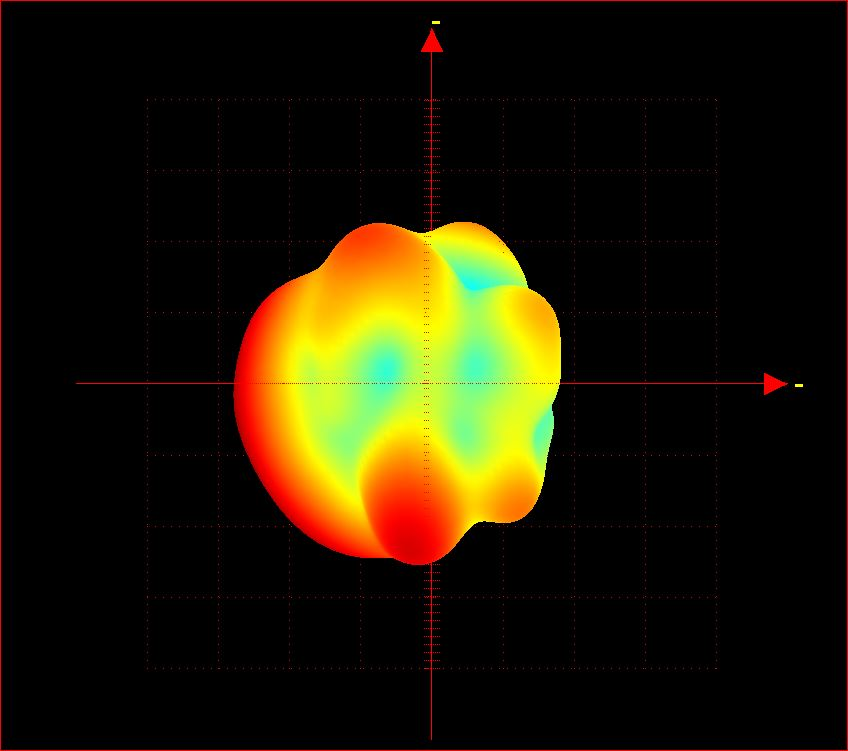
\includegraphics[width=8cm]{content/bilder/Implementierung/min25_0_x_yhinten_zoben.JPG}%
	\caption{3DrichtidiagrammDipolantenne}
	\label{fig:3D Richtdiagramm}
\end{figure}
%%%%%%%%%%%%%%%%%%%%%%%%%%%%%%%%%%%%%%%%%%%%%%%%%%%%%%%%%%%%%%%%%%%
%%%%%%%%%%%%%%%%%%%%%%%%%%%%%%%%%%%%%%%%%%%%%%%%%%%%%%%%%%%%%%%%%%%
\begin{figure}[!h]
	\centering
	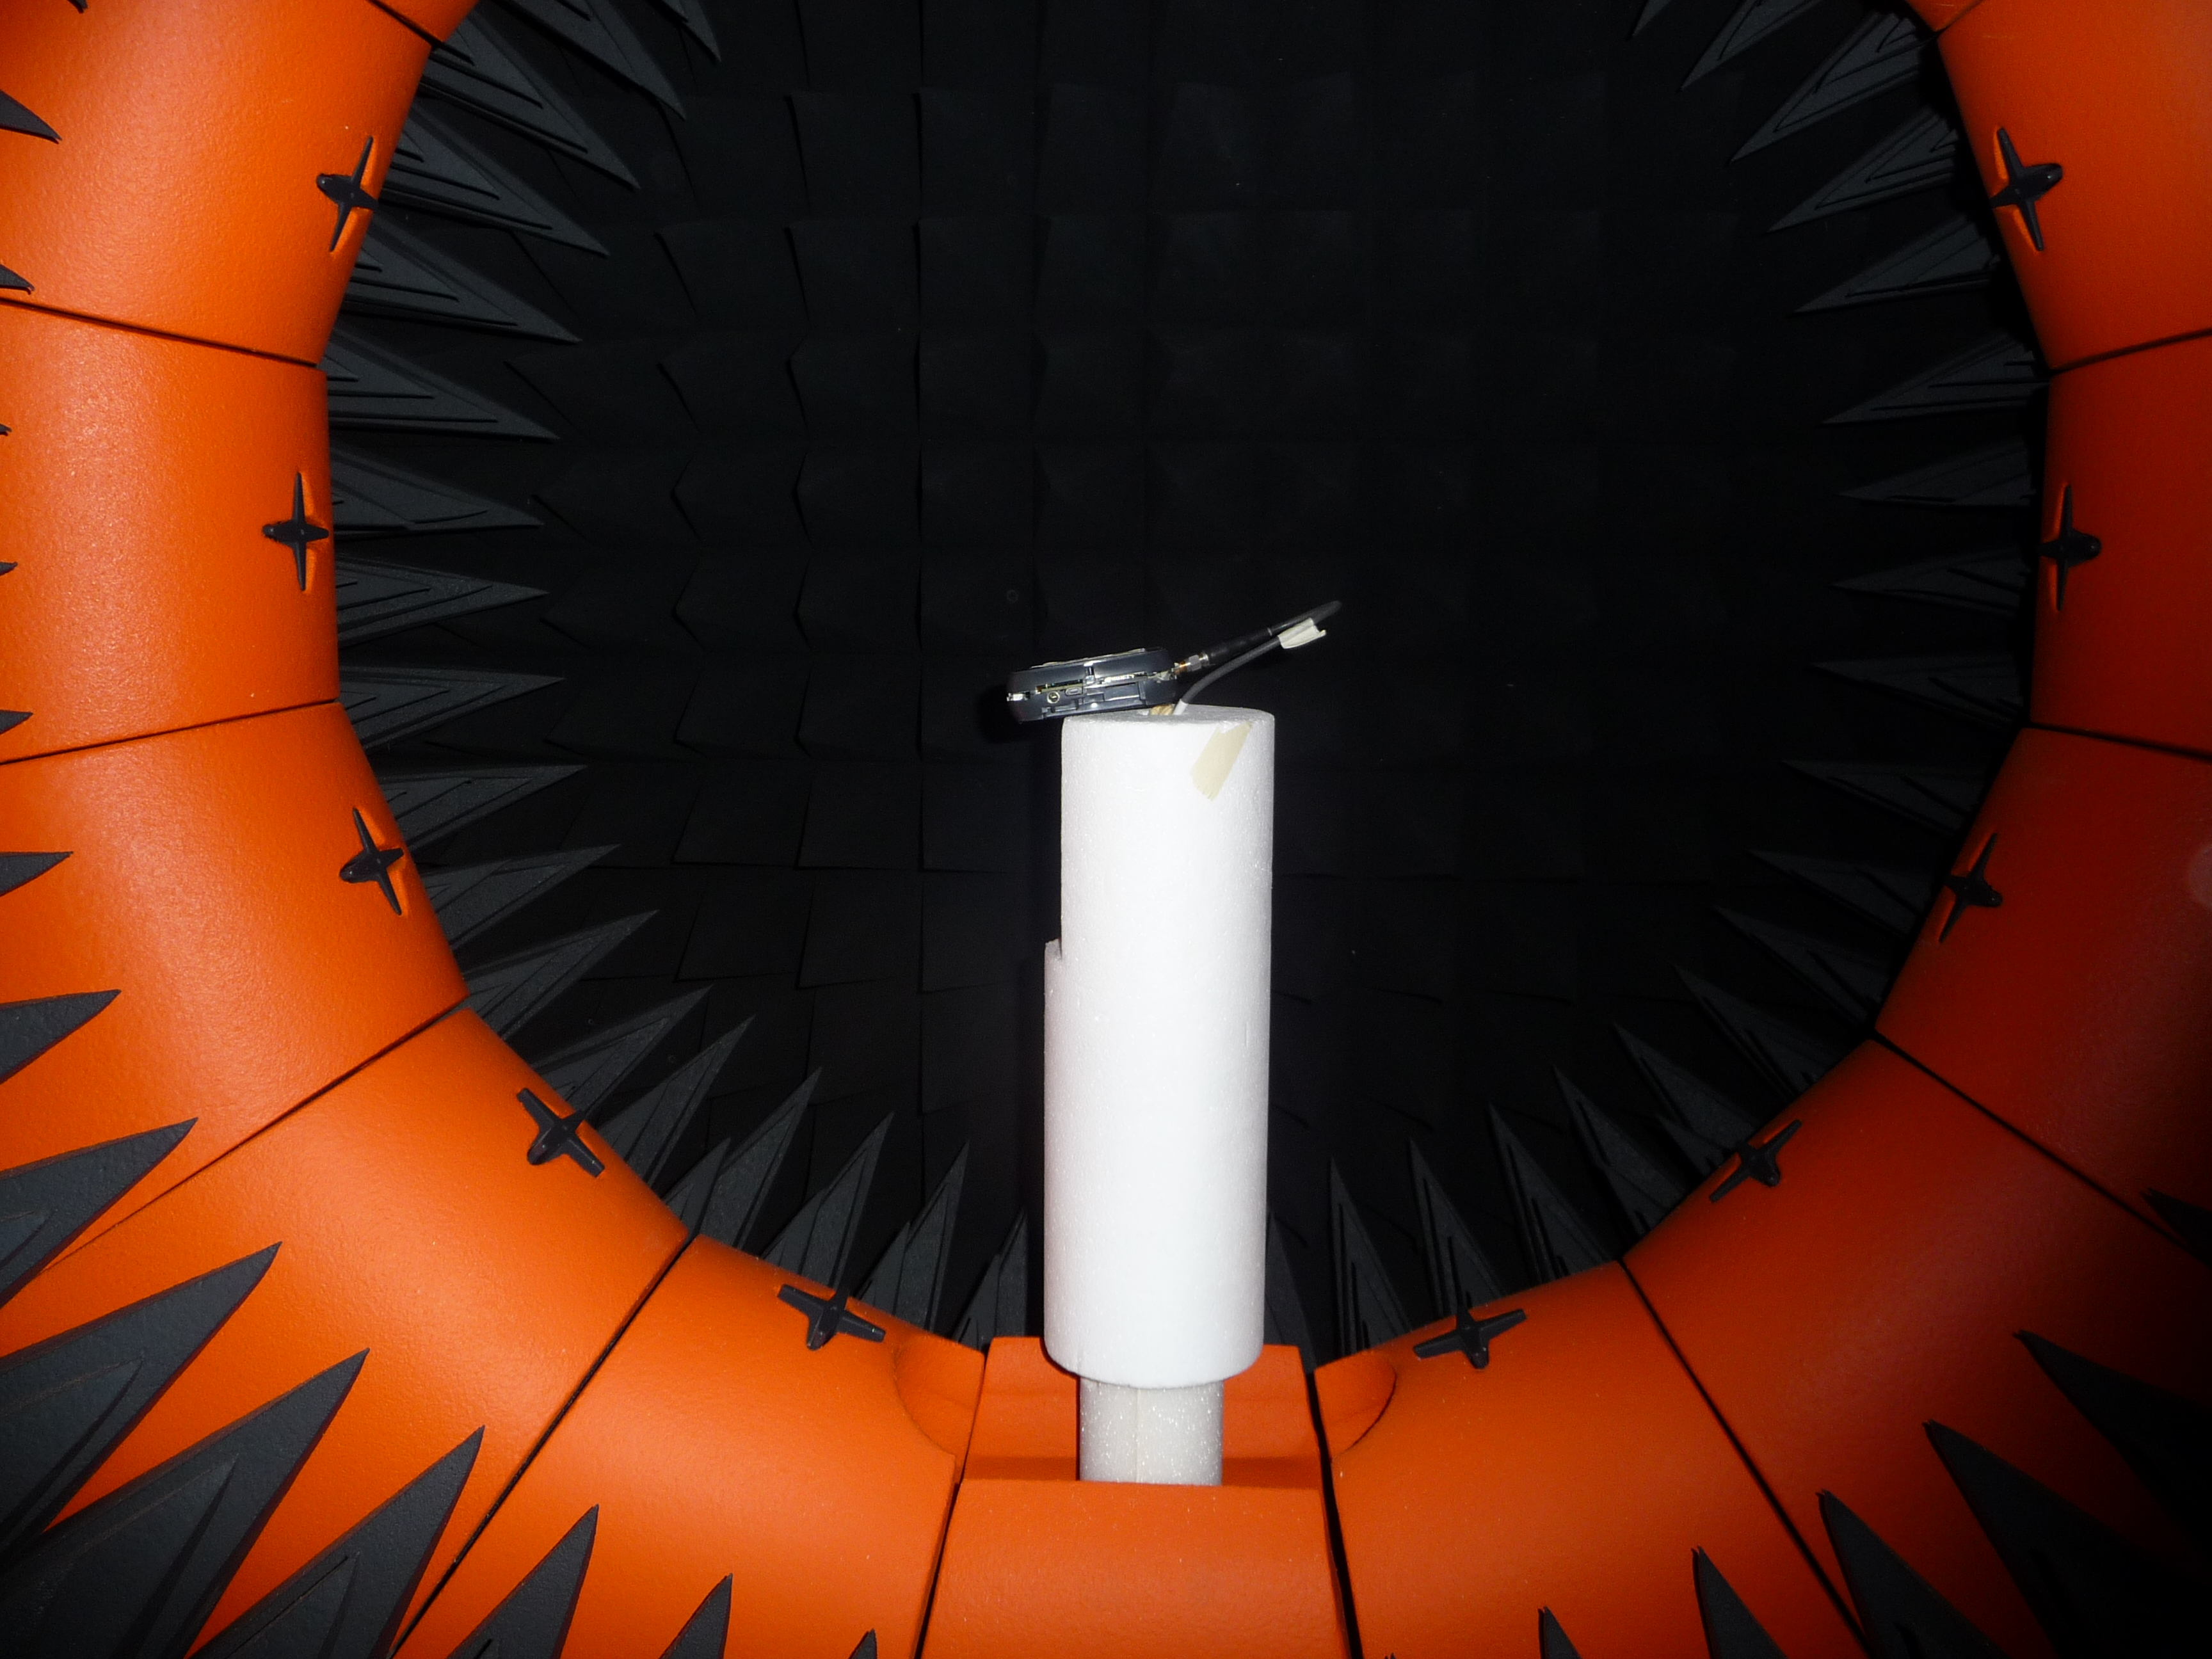
\includegraphics[width=8cm]{content/bilder/Implementierung/Front.JPG}%
	\caption{Versuchsanordnung Front Perspektive im Starlab}
	\label{fig:FrontStarLab}
\end{figure}
%%%%%%%%%%%%%%%%%%%%%%%%%%%%%%%%%%%%%%%%%%%%%%%%%%%%%%%%%%%%%%%%%%%
\newpage
Ein Schnitt durch die xy-Ebende bei z=0 ist in Abbildung \ref{fig:Schnittgemessen} in der oberen Grafik dargestellt. Aus den Simulationen ist zu erwarten, dass die elektromagnetische Feldstärke in Richtung der positiven x-Achse kleiner sein muss als auf der negativen Seite der x-Achse. Da das elektromagnetisch Feld auf die linke Seite (neg.x-Achse) nur durch die Gehäusewand gedämpft wird. Der Schnitt durch die xy-Ebene zeigt einen Schnitt wie in einer Vogelperspektive auf das Gerät. Bei der Messung der Feldstärke im Starlab ist das Gerät wie in der Simulation in der xy-Ebene auf der Höhe z=0 positioniert. Das Display zeigt bei der Messung und der Simulation in die positive z-Richtung.    \\
%\begin{figure}[!ht]
%	\centering
%	\begingroup
%	\inputencoding{latin1}
%	\input{content/bilder/Messung/xyGeraet.tikz}
%	\endgroup
%	\caption{xy-Ebene}\label{fig:xy_gemessen}
%\end{figure}

Ein Schnitt in der xz-Ebene bei y=0 ist in der unteren Grafik von Abbildung \ref{fig:Schnittgemessen} gezeigt. Das Gerät ist in der xy-Ebene positioniert. Das Display zeigt in die Richtung der positiven z-Achse. Die Ausrichtung der Antenne im Gerät ist entlang der y-Achse. Der Dipol ist im Ursprung des Koordinatensystems plaziert. Aus der Theorie sollte jetzt ein Kreis ersichtlich sein. Da ein radiales elektromagetisches Feld um die längsausrichtung des Dipols zu erwarten ist. Die absorbierenden Eigenschaften des Gerätes zeigen jedoch ein starke Reduktion der elektromagnetischen Feldstärke in Richtung der positiven x-Achse, sowie ein reduziertes Feld entlang der negativen x-Achse. Um diese Abbildung zu ploten war es nötig einen offste von 17.6 dB zu den Richtwirkun zu addieren.\\
Um die ensprechenden in der $\varphi$ zu erhalten muss zuerst der $\theta$ Winkel bei -90$^{circ}$ festgehalten werden und $\varphi$ nimmt die elektromagnetische Feldstärkte von $0..\pi$ auf. Anschliessen wird der $\theta$ Winkel bei 90$^{\circ}$ festgehalten  und $\varphi$ nimmt die elektromagnetische Feldstärkte von $0..\pi$ auf. Somit ist die ganze xy-Ebene auf der Höhe z=0 aufgenommen.\\
Der Schnitt in der xz-Eben kann mit festem Winkel $\varphi$ bei 0$^{\circ}$ über den  $\pm \theta$ Bereich aufgenommen werden.
\begin{figure}[!h]
	\centering
	\begingroup
	\inputencoding{latin1}
	% This file was created by matlab2tikz.
%
%The latest updates can be retrieved from
%  http://www.mathworks.com/matlabcentral/fileexchange/22022-matlab2tikz-matlab2tikz
%where you can also make suggestions and rate matlab2tikz.
%
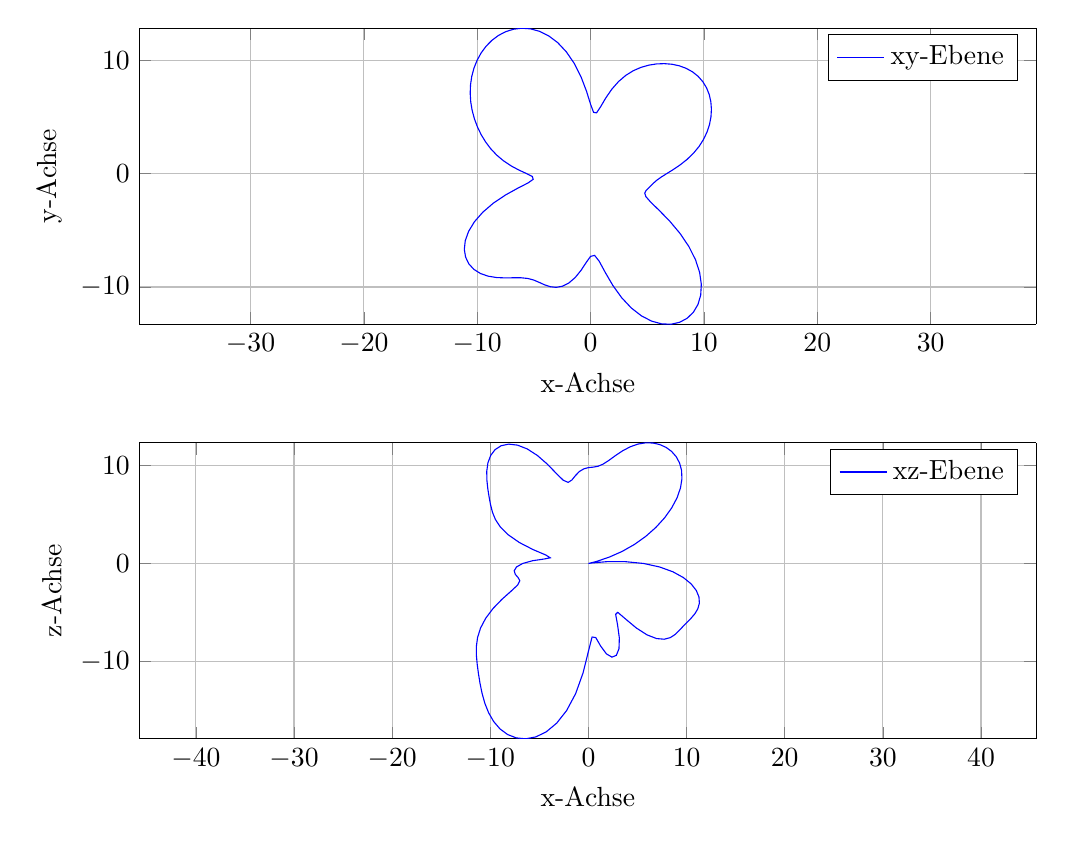
\begin{tikzpicture}

\begin{axis}[%
width=4.484in,
height=1.48in,
at={(0.777in,2.567in)},
scale only axis,
separate axis lines,
every outer x axis line/.append style={black},
every x tick label/.append style={font=\color{black}},
xmin=-39.7978806344427,
xmax=39.3189885799739,
xlabel={x-Achse},
xmajorgrids,
every outer y axis line/.append style={black},
every y tick label/.append style={font=\color{black}},
ymin=-13.2831356744683,
ymax=12.8378951891962,
ylabel={y-Achse},
ymajorgrids,
axis background/.style={fill=white},
legend style={legend cell align=left,align=left,draw=black}
]
\addplot [color=blue,solid]
  table[row sep=crcr]{%
-5.619871535019	6.88235768698034e-16\\
-5.13539941187671	-0.252285995411725\\
-5.06482938714876	-0.498842154080948\\
-5.52511928513371	-0.819574025444295\\
-6.42023039791496	-1.27706322757637\\
-7.50955314367395	-1.88104513934036\\
-8.58532244753228	-2.60432909212068\\
-9.51765446098433	-3.40547121967372\\
-10.2505625547149	-4.24592203213204\\
-10.7627351667713	-5.09039462611558\\
-11.0550569353173	-5.9090510404487\\
-11.1385146358514	-6.67616874766665\\
-11.0254280981749	-7.36695552834882\\
-10.7361608143271	-7.9624795334687\\
-10.2912346035501	-8.44579797104457\\
-9.71619554376366	-8.8062463249902\\
-9.04195760180511	-9.04195760185126\\
-8.30552923785591	-9.16373937227696\\
-7.54699681467832	-9.19604222587177\\
-6.81165880652291	-9.18445869186171\\
-6.13658598548595	-9.1840499480399\\
-5.54076876759112	-9.24421421102729\\
-5.0164748738578	-9.3851643806793\\
-4.53545791137206	-9.58942006413594\\
-4.06172168201249	-9.80586357140556\\
-3.56814084090405	-9.97228559593589\\
-3.04263565105334	-10.0302255315353\\
-2.48728196471192	-9.92978621506686\\
-1.91825450553884	-9.64371662934876\\
-1.35942118201809	-9.16447320014774\\
-0.839527165664564	-8.52386236062131\\
-0.384610554950385	-7.8289277023075\\
3.72266900970547e-11	-7.2946459490993\\
0.354055734367555	-7.2069700394241\\
0.76099870156028	-7.72654948324138\\
1.29170188173944	-8.70794675964638\\
1.96014036122884	-9.85429105039494\\
2.74081405626321	-10.9419430602905\\
3.59592146954104	-11.8541644377876\\
4.48966676500829	-12.5477780183307\\
5.38980352309835	-13.0121367637555\\
6.26846856131452	-13.2535632269825\\
7.09998393803599	-13.2831356744683\\
7.85872561869968	-13.1114915800484\\
8.52262745664405	-12.7550133658514\\
9.06776787324646	-12.2264696196607\\
9.4722857522601	-11.5420135837446\\
9.71351046661139	-10.7172072669825\\
9.76965315521267	-9.7696531550631\\
9.62248973398557	-8.72131632939575\\
9.2584203678348	-7.59818923272191\\
8.67549634485242	-6.43418660373574\\
7.89243601182051	-5.27355714471958\\
6.97638699524198	-4.18148544495084\\
6.05328311298777	-3.23554723269324\\
5.30364519946454	-2.50843736303377\\
4.87477158965361	-2.01919650585457\\
4.77678986043565	-1.70916274159945\\
4.89473466121119	-1.48480152670051\\
5.10056986244105	-1.27762624023851\\
5.32232969747921	-1.05867720032435\\
5.55908800121079	-0.824612808203858\\
5.84323022443261	-0.575507944737531\\
6.21842324270619	-0.305491544306844\\
6.7043037135222	-1.64208081665534e-15\\
7.28138779058552	0.357711644098842\\
7.90136110523392	0.778216143648855\\
8.51281339985814	1.26275658242354\\
9.07506179779524	1.80514202632216\\
9.56433220731451	2.3957405008527\\
9.96329093777777	3.02233126374598\\
10.2719964921601	3.6753791142595\\
10.4918571988236	4.34586954625022\\
10.6210037729137	5.02336066918314\\
10.6596225813826	5.69768697473488\\
10.6081577440118	6.35828506010452\\
10.4645004296223	6.99215564284307\\
10.2267512869281	7.58467567916575\\
9.89896204407976	8.12386820124531\\
9.48380970599508	8.5956240788022\\
8.989735795337	8.98973579538288\\
8.42953212920648	9.30055547937897\\
7.81650652904585	9.524440762994\\
7.16515936630726	9.66109902002675\\
6.49014109296708	9.71318255926234\\
5.80549699388031	9.68588657350462\\
5.11850789165589	9.57605473065038\\
4.43657016617326	9.38033949356579\\
3.76379338878711	9.08660104527841\\
3.10436592256449	8.67612153063455\\
2.46699132795512	8.13258051293959\\
1.86594731706179	7.44927925738695\\
1.32459495835026	6.65918854360031\\
0.873338079735684	5.88756710008339\\
0.528848803956966	5.36949201749774\\
0.265899305899282	5.41250471466588\\
-3.12425291723953e-11	6.1221843103277\\
-0.357165519573225	7.27027117150815\\
-0.841612085236744	8.54503090339449\\
-1.44438656412597	9.73726327921743\\
-2.13905511055011	10.7537562355896\\
-2.89602118781217	11.5615646621569\\
-3.68886148871334	12.1605466208947\\
-4.49486989535147	12.5623197934698\\
-5.29427880626339	12.7815196968349\\
-6.07187222098076	12.8378951891961\\
-6.81324234187685	12.7466798798445\\
-7.50737798624564	12.5253034691377\\
-8.14527998716991	12.1902729684567\\
-8.71993572254039	11.7574722563849\\
-9.22587393957372	11.2417599212595\\
-9.65707918074072	10.6549449377147\\
-10.0116746111118	10.0116746109585\\
-10.2865980532525	9.32322902449111\\
-10.4799413247626	8.60066557466009\\
-10.5912849067743	7.855032237314\\
-10.6210975452244	7.09679049161679\\
-10.5724031566805	6.33685458503991\\
-10.4470922113125	5.58408712479986\\
-10.2502615174658	4.84801264116884\\
-9.98560663122488	4.13617369507158\\
-9.65882793617277	3.45598389679232\\
-9.26797297923333	2.8114088671723\\
-8.81309499083826	2.2075653743954\\
-8.28812938118591	1.64861143670895\\
-7.68819191780966	1.14043554014155\\
-7.0160488269907	0.691020494745552\\
-6.30025278853983	0.309511572109868\\
-5.619871535019	6.88235768698034e-16\\
};
\addlegendentry{xy-Ebene};

\end{axis}

\begin{axis}[%
width=4.484in,
height=1.48in,
at={(0.777in,0.494in)},
scale only axis,
separate axis lines,
every outer x axis line/.append style={black},
every x tick label/.append style={font=\color{black}},
xmin=-45.74965043919,
xmax=45.627735202645,
xlabel={x-Achse},
xmajorgrids,
every outer y axis line/.append style={black},
every y tick label/.append style={font=\color{black}},
ymin=-17.8714260057326,
ymax=12.2975067931959,
ylabel={z-Achse},
ymajorgrids,
axis background/.style={fill=white},
legend style={legend cell align=left,align=left,draw=black}
]
\addplot [color=blue,solid]
  table[row sep=crcr]{%
9.11969905341734e-11	-8.93485025483866\\
-0.547612181295438	-11.1469020325363\\
-1.30644250147935	-13.264533323878\\
-2.22309191890158	-14.9868683690143\\
-3.23710378260406	-16.2740196829566\\
-4.29758335773247	-17.1569144914293\\
-5.36206729836429	-17.6763669683003\\
-6.39449847296901	-17.8714260057326\\
-7.36373523191796	-17.77762946707\\
-8.24370135014945	-17.4298420745342\\
-9.01269835389525	-16.8615726566521\\
-9.65712201459447	-16.1119346990514\\
-10.1712108289648	-15.2222927385399\\
-10.5608975880847	-14.2397219829766\\
-10.8457925847976	-13.215636501913\\
-11.053377270834	-12.1955224758874\\
-11.2118454529987	-11.2118454531704\\
-11.3369009923115	-10.2751681202448\\
-11.4181151721281	-9.37060495362239\\
-11.4227283695084	-8.47167273595405\\
-11.3007076628774	-7.55089145300298\\
-11.0009168163071	-6.59369578858987\\
-10.4838275944297	-5.6037225963642\\
-9.73927882518462	-4.60633582682547\\
-8.81823850212206	-3.65263398388547\\
-7.88339354073699	-2.82072331241613\\
-7.20396005248313	-2.18529739100488\\
-6.99432111024179	-1.75198623382895\\
-7.17526624016463	-1.42724919408035\\
-7.45660381952669	-1.10608269100847\\
-7.56510061023217	-0.745097375490363\\
-7.33788375787576	-0.360487112945744\\
-6.7043037135222	-3.42152343239187e-11\\
-5.69644430609545	0.27984836354608\\
-4.55291499138621	0.448422986730577\\
-3.89491064322866	0.577755416469261\\
-4.34919131850486	0.865107941556732\\
-5.64062697234519	1.41290350407482\\
-7.04262690287729	2.13635751503205\\
-8.1771350247479	2.92582569589471\\
-8.97576552608844	3.71788381354646\\
-9.48223758191485	4.48476437269101\\
-9.78565302100887	5.23054051192107\\
-9.97513534167612	5.97886603360216\\
-10.1222369757389	6.76346251583093\\
-10.2546257026021	7.60534875469799\\
-10.3505168407088	8.49444964566792\\
-10.3634080921611	9.39284558590508\\
-10.2466753547619	10.2466753547096\\
-9.96926803586775	10.9993922597653\\
-9.51867201977703	11.5985354143698\\
-8.89981901670096	12.0000168013096\\
-8.12831076286041	12.1648767296991\\
-7.22991051673073	12.0623769635312\\
-6.24074526760137	11.6756131872752\\
-5.20732747820439	11.0099689102753\\
-4.19500385276841	10.1276351955243\\
-3.28924490203915	9.19282366396339\\
-2.57453378423401	8.4871004807292\\
-2.07025631112067	8.26492648381575\\
-1.69186098547946	8.50555954745951\\
-1.32842474419331	8.95551218697102\\
-0.923363560628339	9.37506756121862\\
-0.473943259620469	9.64733667735239\\
-5.98267499453569e-16	9.77044973081391\\
0.482405350601725	9.81958649636226\\
0.975880853203647	9.90828458105723\\
1.50309486764442	10.1330425108405\\
2.09201221236382	10.5172556131911\\
2.75555477689471	11.0007913178798\\
3.48423755473685	11.4859919131261\\
4.25492980840347	11.8917321744409\\
5.04039702528872	12.1685948581531\\
5.81628754444984	12.2975067931959\\
6.56330025184386	12.2790711183646\\
7.26499089146219	12.1209050328695\\
7.90617444315454	11.8324262334954\\
8.46972723305956	11.4201051626441\\
8.93662415801328	10.8893080427892\\
9.28300138357769	10.2422136909701\\
9.48735450143698	9.48735450138857\\
9.52313505323396	8.6312664958554\\
9.37441432381955	7.69338301234627\\
9.02794382166376	6.69557946753254\\
8.48356084122461	5.66853412816938\\
7.75364028834732	4.64735314047173\\
6.86017624813366	3.66684059896111\\
5.83413707922204	2.75934133607807\\
4.68789584140558	1.9417900364816\\
3.42845608445968	1.22672120232819\\
2.07493250522317	0.629423894215773\\
0.77303712804341	0.193635720345881\\
0	0\\
0.375052798261174	0.0556338271929451\\
1.8532379543519	0.182528006823146\\
3.76149386545658	0.184790343971285\\
5.619871535019	-2.86801755283784e-11\\
7.24915752742728	-0.356128272752533\\
8.60116319283983	-0.847140633196758\\
9.67058811200071	-1.43449623735477\\
10.4636603071623	-2.08135144267279\\
10.9878740216496	-2.75231916315483\\
11.2596415100906	-3.41557491107547\\
11.3008131329635	-4.04349559471928\\
11.1457798881788	-4.61673319299224\\
10.8413627358251	-5.12758269662694\\
10.4493374426103	-5.58528722613687\\
10.0290528660722	-6.01118295418253\\
9.62143436211023	-6.42883690630656\\
9.23177478452401	-6.84675081264194\\
8.82384294616145	-7.24154075999528\\
8.33778943768367	-7.55693185302602\\
7.71994172349886	-7.71994172361705\\
6.93484400382598	-7.65142126638472\\
5.97422475460088	-7.2796139258834\\
4.87801709468061	-6.57724465909308\\
3.7825735664962	-5.66102139681324\\
2.98263543363491	-4.97622658854028\\
2.77096316856667	-5.18410746272236\\
2.96762440901681	-6.27451463713662\\
3.14717568021532	-7.59795421053852\\
3.10909430230828	-8.68933646687514\\
2.84032868633189	-9.36330884647951\\
2.39116611984348	-9.54607025344666\\
1.83287598627931	-9.21448982804405\\
1.25089245951515	-8.43283198285789\\
0.74378307460804	-7.55175629061597\\
0.368196961731472	-7.49482133759175\\
-9.11958963305968e-11	-8.93485025483866\\
9.11969905341734e-11	-8.93485025483866\\
};
\addlegendentry{xz-Ebene};

\end{axis}
\end{tikzpicture}%
	\endgroup
	\caption{Schnitte durch das 3D Richtdiagramm}
	\label{fig:Schnittgemessen}
\end{figure}
\newpage
Die Effizienz der Dipolantenne ist in Abhängigkeit der Frequenz in der Abbildung \ref{fig:Effizienz_gemessen} gezeigt. Sie zeigt bei 2.45GHz eine $\eta_{tot}$ von 49$\%$. Über eine Bandbreite von 100 MHz nimmt die Effizienz Werte im Bereich von 47$\%$ bis 56.3$\%$ an.\\
\begin{figure}[!h]
	\centering
	\begingroup
	\inputencoding{latin1}
	% This file was created by matlab2tikz.
%
%The latest updates can be retrieved from
%  http://www.mathworks.com/matlabcentral/fileexchange/22022-matlab2tikz-matlab2tikz
%where you can also make suggestions and rate matlab2tikz.
%
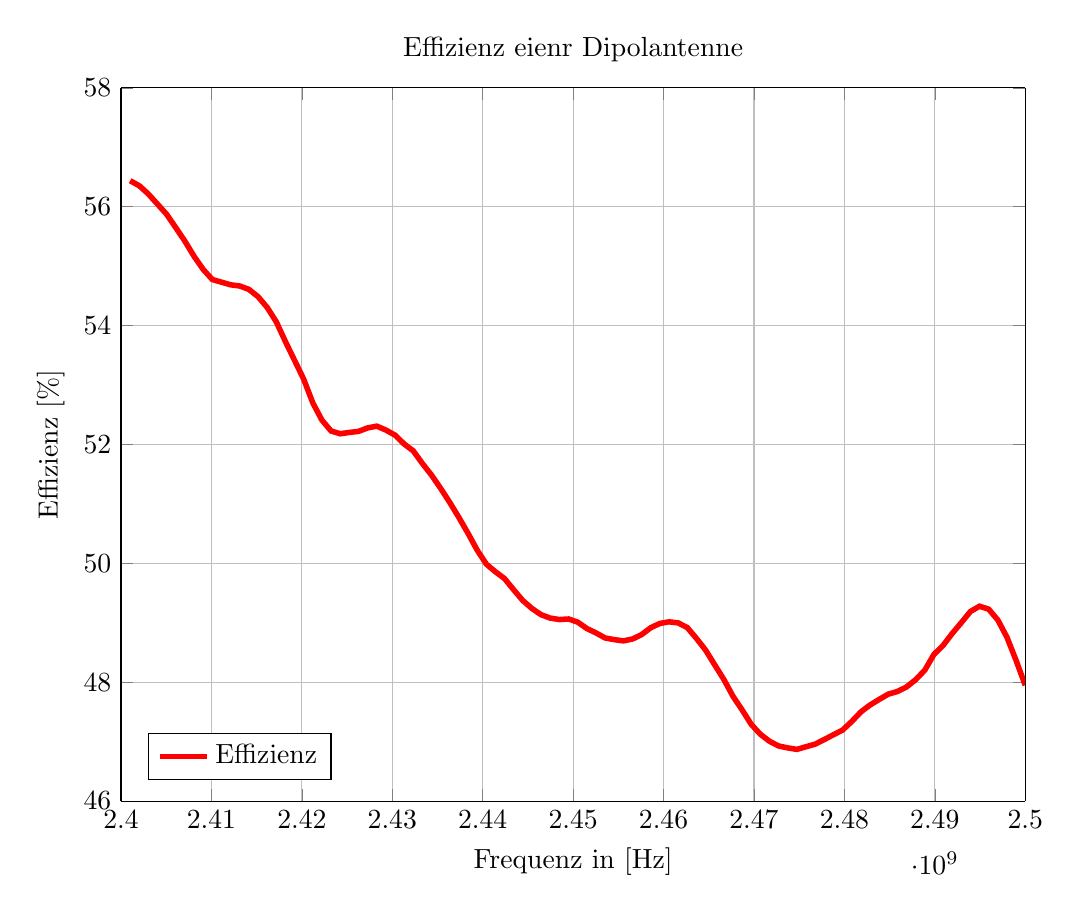
\begin{tikzpicture}

\begin{axis}[%
width=4.521in,
height=3.566in,
at={(0.758in,0.481in)},
scale only axis,
separate axis lines,
every outer x axis line/.append style={black},
every x tick label/.append style={font=\color{black}},
xmin=2400000000,
xmax=2500000000,
xlabel={Frequenz in [Hz]},
xmajorgrids,
every outer y axis line/.append style={black},
every y tick label/.append style={font=\color{black}},
ymin=46,
ymax=58,
ylabel={Effizienz [\%]},
ymajorgrids,
axis background/.style={fill=white},
title={Effizienz eienr Dipolantenne},
legend style={at={(0.03,0.03)},anchor=south west,legend cell align=left,align=left,draw=black}
]
\addplot [color=red,solid,line width=2.0pt]
  table[row sep=crcr]{%
2401010101	56.4375042915344\\
2402020202	56.3531458377838\\
2403030303	56.2125742435455\\
2404040404	56.0422480106354\\
2405050505	55.8718800544739\\
2406060606	55.6469202041626\\
2407070707	55.418872833252\\
2408080808	55.165308713913\\
2409090909	54.9443542957306\\
2410101010	54.7752261161804\\
2411111111	54.7305941581726\\
2412121212	54.6864569187164\\
2413131313	54.6665072441101\\
2414141414	54.6095192432404\\
2415151515	54.4872283935547\\
2416161616	54.3057501316071\\
2417171717	54.0638506412506\\
2418181818	53.7307322025299\\
2419191919	53.4151136875153\\
2420202020	53.0986845493317\\
2421212121	52.6989936828613\\
2422222222	52.4086833000183\\
2423232323	52.2269546985626\\
2424242424	52.1802008152008\\
2425252525	52.2026240825653\\
2426262626	52.2199869155884\\
2427272727	52.2787272930145\\
2428282828	52.308177947998\\
2429292929	52.2423028945923\\
2430303030	52.1572828292847\\
2431313131	52.0078897476196\\
2432323232	51.8917977809906\\
2433333333	51.6792297363281\\
2434343434	51.483166217804\\
2435353535	51.2607336044312\\
2436363636	51.0222971439362\\
2437373737	50.7695019245148\\
2438383838	50.503146648407\\
2439393939	50.2213001251221\\
2440404040	49.9863803386688\\
2441414141	49.8573243618011\\
2442424242	49.7420459985733\\
2443434343	49.5531976222992\\
2444444444	49.3724018335342\\
2445454545	49.2388904094696\\
2446464646	49.1352200508118\\
2447474747	49.0781038999558\\
2448484848	49.0543007850647\\
2449494949	49.0636646747589\\
2450505050	49.0110695362091\\
2451515151	48.903015255928\\
2452525252	48.8299459218979\\
2453535353	48.7446904182434\\
2454545454	48.7163454294205\\
2455555555	48.6952841281891\\
2456565656	48.7268656492233\\
2457575757	48.8009363412857\\
2458585858	48.9171475172043\\
2459595959	48.9889591932297\\
2460606060	49.0157067775726\\
2461616161	48.9983528852463\\
2462626262	48.9188820123673\\
2463636363	48.7371891736984\\
2464646464	48.5411763191223\\
2465656565	48.2924193143845\\
2466666666	48.0470031499863\\
2467676767	47.7638095617294\\
2468686868	47.5343286991119\\
2469696969	47.2913831472397\\
2470707070	47.1245557069778\\
2471717171	47.0063269138336\\
2472727272	46.9269156455994\\
2473737373	46.8947410583496\\
2474747474	46.869620680809\\
2475757575	46.9143569469452\\
2476767676	46.9577997922897\\
2477777777	47.0354378223419\\
2478787878	47.1161991357803\\
2479797979	47.1948862075806\\
2480808080	47.3383545875549\\
2481818181	47.498819231987\\
2482828282	47.6154237985611\\
2483838383	47.7093458175659\\
2484848484	47.7990716695786\\
2485858585	47.843337059021\\
2486868686	47.9196608066559\\
2487878787	48.0419963598251\\
2488888888	48.2016503810883\\
2489898989	48.4668105840683\\
2490909090	48.6176282167435\\
2491919191	48.8188236951828\\
2492929292	49.0015745162964\\
2493939393	49.1898447275162\\
2494949494	49.2786079645157\\
2495959595	49.2282181978226\\
2496969696	49.0464746952057\\
2497979797	48.7556308507919\\
2498989898	48.3665227890015\\
2500000000	47.9483038187027\\
};
\addlegendentry{Effizienz};

\end{axis}
\end{tikzpicture}%
	\endgroup
	\caption{xy-Ebene}\label{fig:Effizienz_gemessen}
\end{figure}



